\section*{Introduction}

Qualisys is a Swedish motion capture system. The company has developed multiple camera types and software which are able to capture real-time motion of fast moving objects with great precision. Qualisys has features such as capturing 2D, 3D and 6DOF data in real-time with frequencies up to 340Hz. The system tracks small spherical markers placed on an object that will be tracked. The data will be logged and can be analyzed. It’s used in Medical, Engineering, Sport and research applications, such as quadcopters and VR projects \cite{QTM}.
\\
Qualisys Tracking Manager(QTM) is the software used by the motion capture system Qualisys at KIC. This report explains what it is, how it works and why it is used in this bachelors project. \\

\begin{figure}[h]
          \centering
            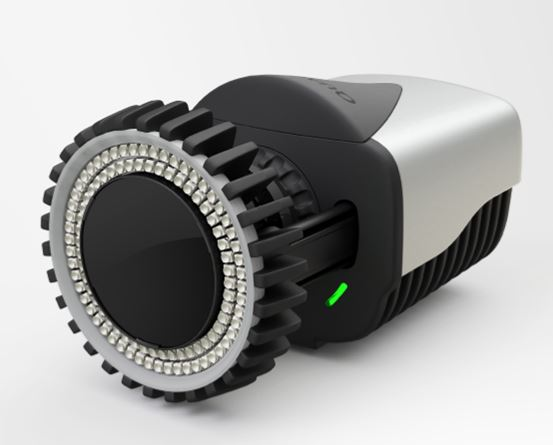
\includegraphics[scale = 0.33]{VAPIQ-PICTURES/m3}
                \caption{Miqus 3}
                \label{m3}
            \label{dir}
\end{figure}


% In this project the Qualisys Tracking Manager(QTM) system is being utilized and this chapter explains what it is, how it works and why  are using it in this project. \\
% \\
% Qualisys is a Sdish motion capture system. The company have developed multiple camera types and software which are able to capture real-time motion of fast moving objects with great precision. Qualisys have features such as capturing 2D, 3D and 6DOF data in real time with low latency. The system tracks small spherical markers placed on the object that will be tracked. The data will be logged and can be analysed. It is used in Medical, Engineering, Sport and research applications, such as quadcopters and VR projects \cite{QTM}.
